\documentclass[a4paper]{article}

%% Language and font encodings
\usepackage[frenchb]{babel}
\usepackage[utf8x]{inputenc}
\usepackage[T1]{fontenc}
\usepackage{minted}
\usepackage{graphicx}

%% Sets page size and margins
\usepackage[a4paper,top=3cm,bottom=2cm,left=3cm,right=3cm,marginparwidth=1.75cm]{geometry}
\setlength{\parskip}{.5em}

%% Useful packages

\title{Projet Reseau : Morpion aveugle}
\author{COUVY Julien, LAMARQUE Gauthier}

\begin{document}
\maketitle

\section{Introduction}
L'objectif de ce projet était de mettre en réseau un jeu de morpion aveugle avec une architecture client-serveur similaire à celle vue dans le TP sur le serveur de chat. Nous avons donc implementé une architecture TCP écrite en Python avec la méthode select().

\section{Structure}

Afin de réaliser cette architecture, nous avons décidé de la stucturer avec des classes.
Ces classes sont les suivantes:
\begin{itemize}
\item la classe User,
\item la classe Game,
\item la classe Room.
\end{itemize}
\bigskip

La classe User représente un client (dans le modèle serveur/client). Cette classe contient les attributs suivants:
la socket associée au client,
un nom qui peut être modifié par le client ("Guest[0...9999] par défaut),
et l'IP du client que l'on obtient lors de la connexion.

La classe Game représente un salon de jeu, où l'on peut faire une partie de morpion ou observer une partie en cours.
Elle contient les attributs suivants:
l'identifiant du salon de jeu,
une paire de joueurs,
une liste d'observateurs,
trois grilles aux contenus différents:
	la première contient les coups joués par le Joueur 1,
	la deuxième les coups joués par le Joueur 2,
	et enfin la dernière contient tous les coups joués et est envoyée aux observateurs présents.
un entier indiquant le tour de jeu.

La classe Room est un salon d'accueil où les clients sont envoyés à la connexion. Depuis ce salon, les clients peuvent rejoindre un salon de jeu, ou effectuer diverses actions comme changer de pseudonyme, obtenir la liste des salons de jeu ou des utilisateurs présents dans le salon d'accueil.
Elle contient les attributs suivants:
une liste de clients,
une liste de salons de jeu (3 dans notre implémentation, choix arbitraire).

\subsection{Pourquoi cette structure?}

Nous avons choisi cette structure car nous avions en tête de réaliser
des parties multiples observables, et nous pensions que cette
structure pouvait remplir ces objectifs. Ce niveau d'abstraction nous
permet aussi d'avoir un code peu redondant, plus modulaire et plus
facile a comprendre. En effet, l'utilisation de classes permet de
différencier aisément les diverses entités que l'on manipule, et de
faciliter l'imbrication de ces entités entre-elles (par exemple :
ajouter un joueur dans un salon de jeu attenant au salon d'accueil).

\newpage
\subsection{Aperçu}

\begin{figure}[h]
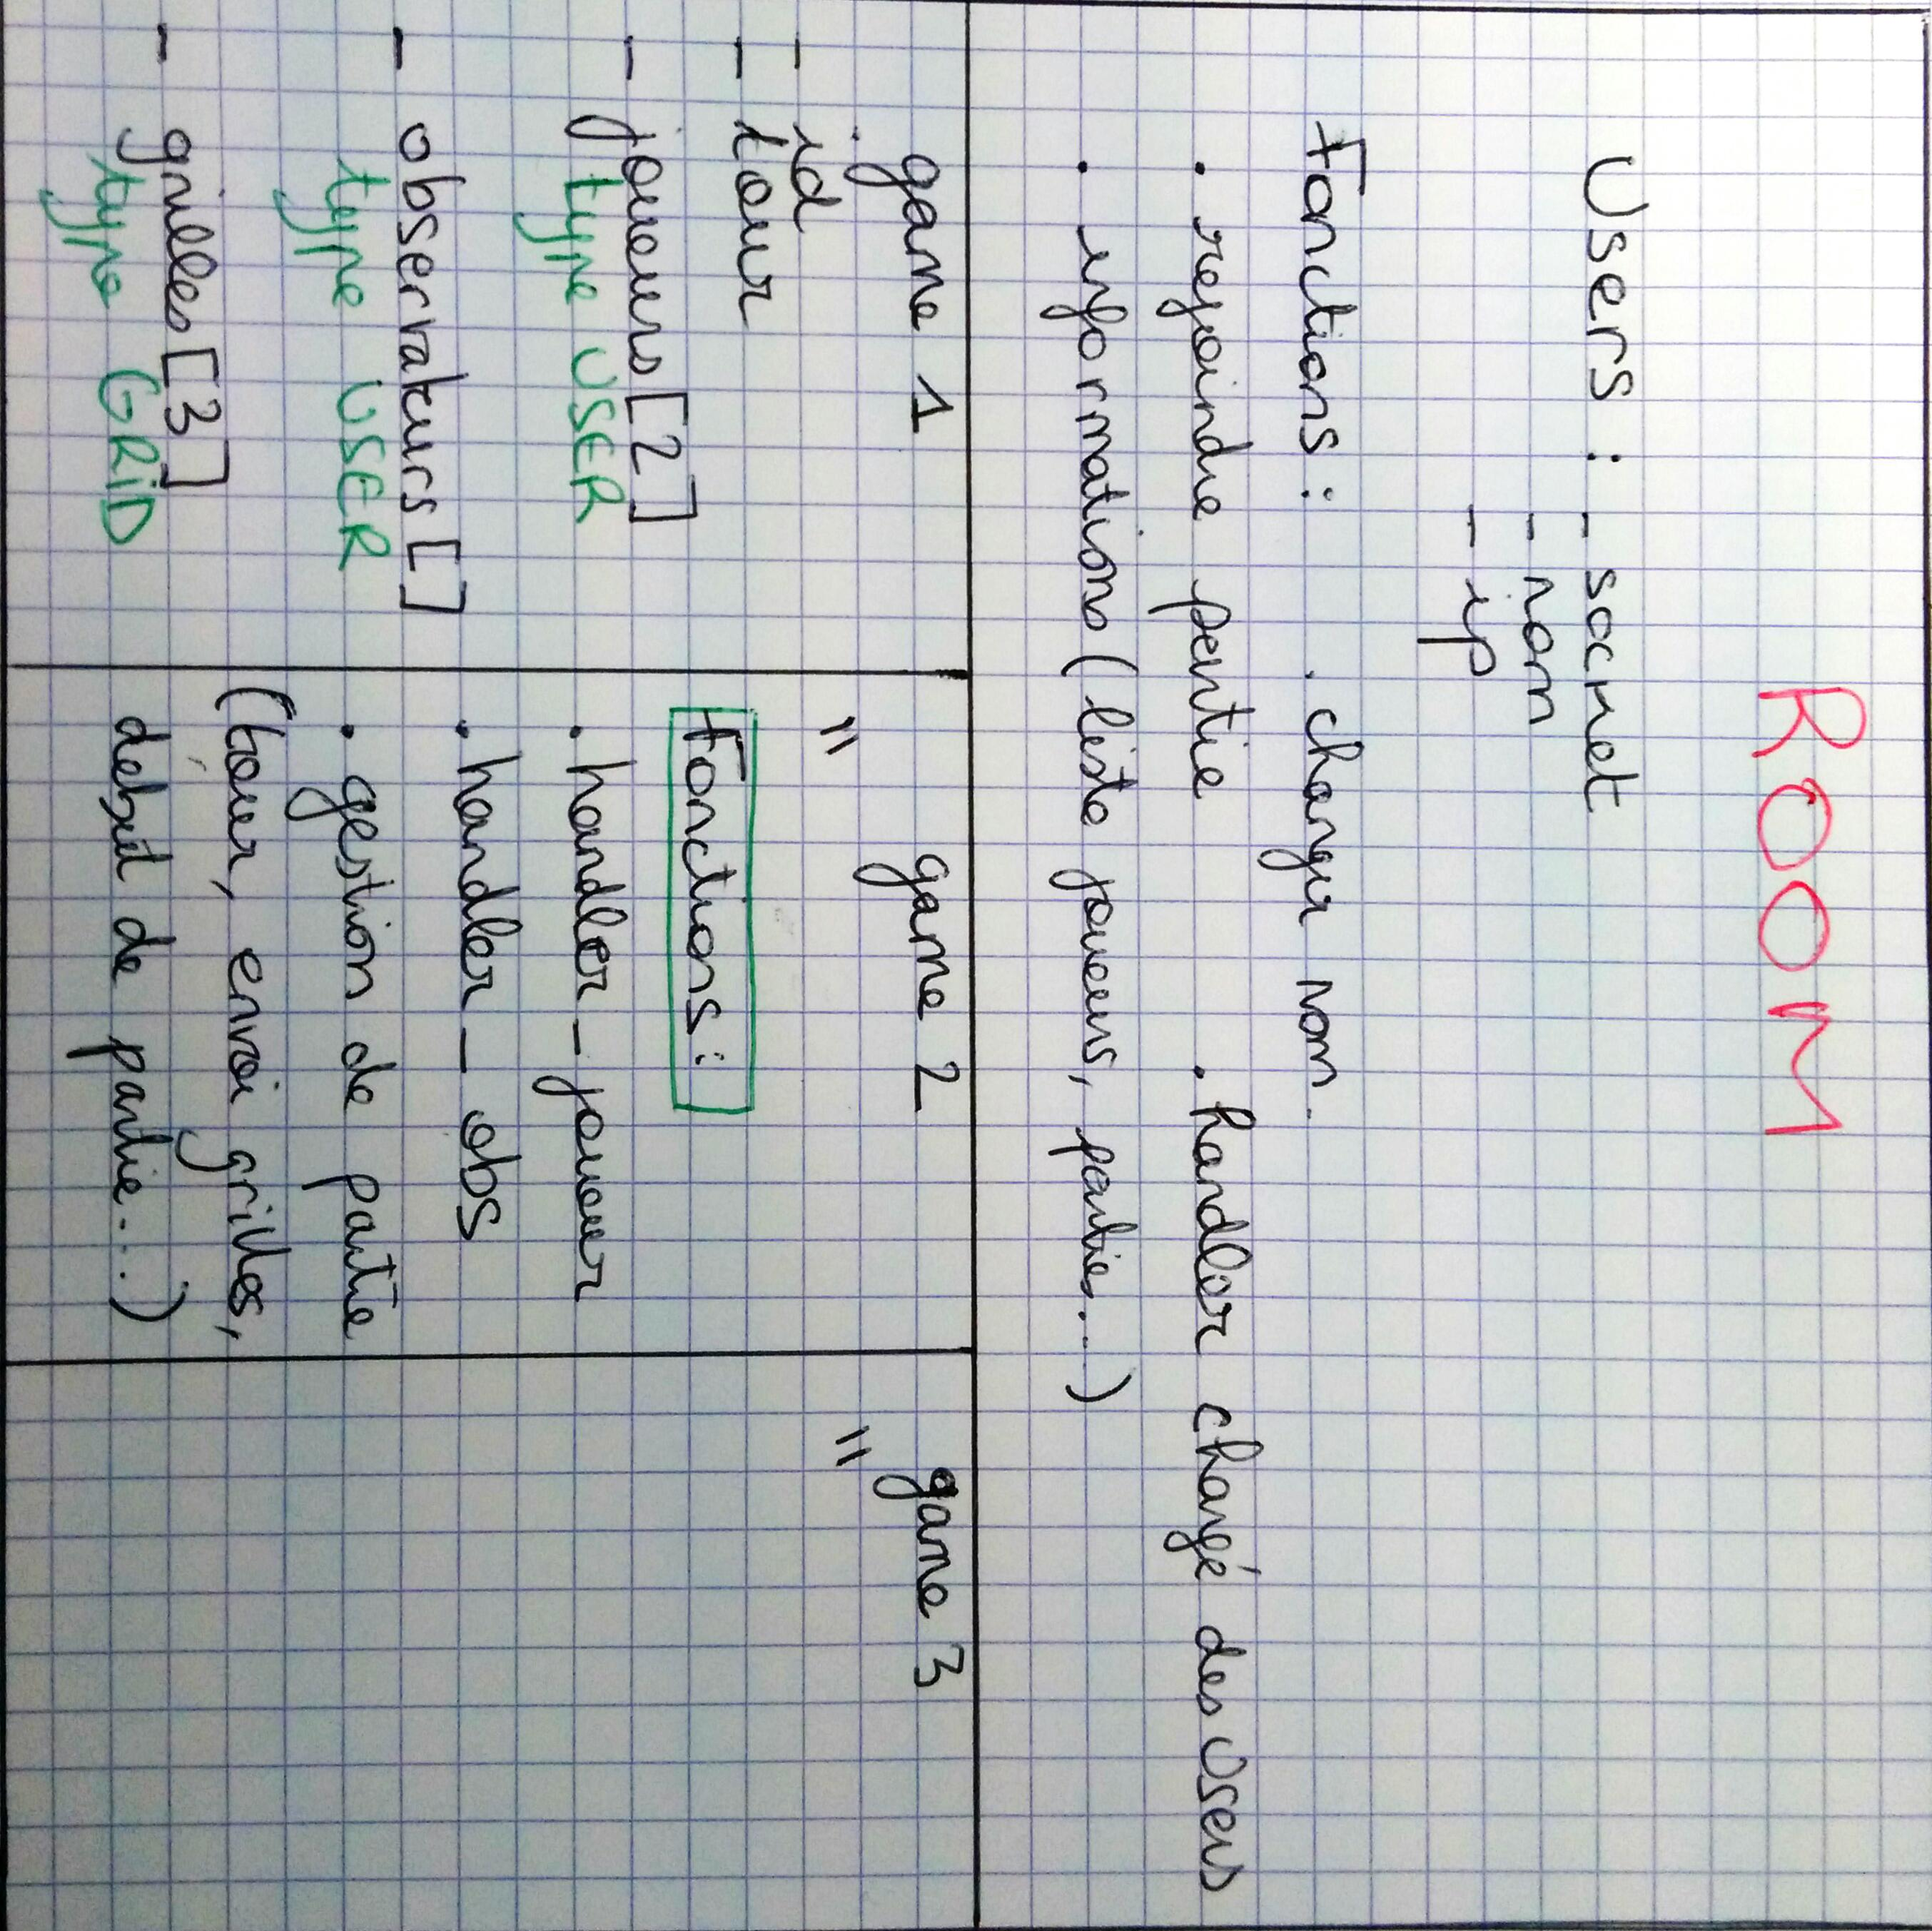
\includegraphics[angle=90,width=\textwidth]{Office_Lens_20161223-105104.jpg}
\end{figure}



\section{Protocole de communication}

Pour que les clients et le serveur puissent communiquer, nous avons établi un protocole permettant à chacun de recevoir et traiter des commandes. Conforme au sujet, le client doit réaliser les affichages. Le protocole est de la forme suivante:
\begin{minted}{bash}
"PREFIXE <contenu>DELIMITEUR"
Exemple: 'GRID 00000000$' envoie une grille vide.
\end{minted}

Le préfixe de la commande est une petite chaîne de caractères majuscules qui permet au client de savoir quel est le type de la commande reçue. Le contenu lui dépend du type de la commande, il peut être inexistant sur certaines commandes.
Le caractère '\$' nous sert de délimiteur. En effet, avec un serveur implémenté en TCP, les transferts d'informations se font par flux de données c'est à dire que l'on remplit un buffer de taille définie (4096 dans notre cas); c'est pourquoi nous avons choisi d'utiliser un délimiteur de commande permettant au client de différencier les commandes et les exécuter dans le bon ordre.

\section{Fonctionnalités}

Comme précisé dans le sujet, le serveur et le client utilisent le même fichier pour s'exécuter. Seul le nombre d'argument change. En effet le client doit renseigner une adresse à laquelle se connecter alors que le serveur n'a pas besoin d'ajouter d'arguments.

\begin{minted}{bash}
$> python3 tictactoe.py (serveur)
$> python3 tictactoe.py localhost (client - içi l'adresse est la boucle locale)
\end{minted}

Nous avons séparé les codes des clients et du serveur dans des fichiers distincts que nous importons dans le main responsable de lancer les bon programmes (plus ergonomique et modulaire).
A la connexion, le client se retrouve dans le salon d'accueil (Room dans le code), et on lui donne la liste des commandes possibles, c'est à dire:
changer de pseudonyme,
obtenir la liste des autres clients ou des parties
enfin rejoindre une partie.
Les entrées client sont gérées par un processus léger (thread) car la fonction "input()" est bloquante, c'est à dire que tant qu'il n'y a pas d'entrée client, on ne peut rien afficher. L'utilisation du processus léger permet d'afficher au client les divers messages du serveur tout en assurant une possible entrée clavier.


À partir de là, l'utilisateur à la possibilité de se rendre dans un des trois salons de jeu disponibles. Lorsqu'un utilisateur rejoint un salon de jeu, il est automatiquement considéré comme un observateur. Il lui est possible de jouer une partie si aucune partie est en cours dans le salon, et si il reste une place de joueur libre, en entrant la commande "play". Si deux utilisateurs ont décidé de jouer, alors une partie débute, le serveur gère l'envoi des grilles aux personnes correspondantes et gère aussi le bon déroulement de la partie. A la fin d'une partie, les joueurs sont replacés parmi les observateurs.


Grâce aux différents salons de jeu, il est possible d'avoir des parties simultanées (en l'occurence trois, choix arbitraire). De plus, lorqu'un joueur est deconnecté pendant une partie (et seulement dans ce cas là), la partie est mise en pause, l'utilisateur est enregistré pour une durée limitée par le serveur. Pendant cette période, il est possible pour le joueur de se reconnecter, et grâce à l'adresse IP de l'utilisateur, le serveur peut le reconnaître et le remettre dans sa position de joueur, et reprendre le cours de la partie.


Si le délai de reconnexion est passé, le joueur restant remporte la partie puis il est replacé parmi les observateurs. Le serveur oublie l'utilisateur deconnecté. Si celui se reconnecte, il sera considéré comme quelconque et entrera dans le salon d'accueil.

\end{document}